\documentclass{beamer}
\usepackage{sdp}

\title{Потоци и файлове}

\subtitle{(преговор)}

\date{17 октомври 2017 г.}

\titlegraphic{
\includegraphics[height=0.2\textheight]{images/stream.jpg}\hspace{5ex}
              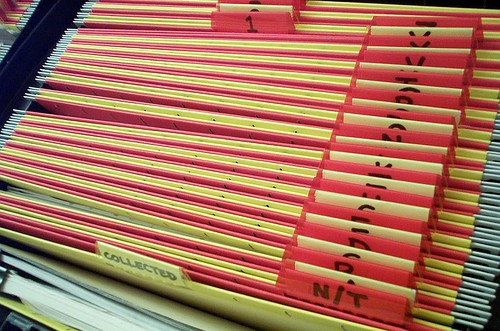
\includegraphics[height=0.2\textheight]{images/files.jpg}}

\usetikzlibrary{arrows.meta,patterns,snakes,math}

\tikzset{
  pointer/.style={-{Stealth}},
  arraynodes/.style={
    rectangle,
    minimum width=3.5ex,
    minimum height=1.5em,
    text height=0.75em,
    text depth=0.25em,
    fill=diagramblue,
    draw=black,
    font=\ttfamily
  },
  array/.style={
    matrix of nodes,
    nodes=arraynodes,
    column sep=-\pgflinewidth,
    inner sep=0pt,
    nodes in empty cells,
    ampersand replacement=\&,
  }
}

\begin{document}

\begin{frame}
  \titlepage
\end{frame}

\section{Поточна обработка на данни}

\begin{frame}
  \frametitle{Абстракцията поток}

  \begin{center}
    производител
    $\longrightarrow$ 
\includegraphics[width=0.4\textwidth,valign=c]{images/abstract_stream.pdf}
    $\longrightarrow$ консуматор
  \end{center}
\end{frame}


\begin{frame}
  \frametitle{Поточен буфер}

  \begin{itemize}[<+->]
  \item Какво представлява буферът?
  \item Кога е нужен буфер?
  \item Кога буферът вреди?
  \end{itemize}
  \vspace{2em}
  \onslide<+->
  \begin{tikzpicture}
    \matrix[array] {
      \tt
      H\& e\& l\& l\& o\& ,\&  \& w\& o\& r\& l\& d\& !\& \textbackslash n\\
    };
  \end{tikzpicture}
\end{frame}

\section{Работа с потоци}

\begin{frame}[fragile]
  \frametitle{Стандартни потоци и пренасочване}

  \begin{itemize}[<+->]
  \item Стандартен изходен поток \lst{cout} (\lst{stdout})
    \begin{itemize}[<.->]
    \item Пренасочване на изхода:
    \item \lst!ls > filelist.txt!
    \end{itemize}
  \item Стандартен входен поток \lst{cin} (\lst{stdin})
    \begin{itemize}[<.->]
    \item Пренасочване на вход и на изход:
    \item \lst!grep password < email.txt > password.txt!
    \end{itemize}
  \item Стандартен поток за грешки \lst{cerr} (\lst{stderr})
    \begin{itemize}[<.->]
    \item Пренасочване на изход за грешки:
    \item \lst!mv *.dat /data 2> errors.txt!
    \end{itemize}
  \item Стандартен поток за дневник \lst{clog} (отново \lst{stderr})
  \end{itemize}
\end{frame}

\begin{frame}[fragile]
  \frametitle{Форматиран и неформатиран вход/изход}

  \begin{itemize}[<+->]
  \item Текстова и двоична информация
  \item ASCII (\lst!char!)
  \item Служебни символи
  \item Кодиращи таблици
  \item Unicode (\lst!wchar_t!)
  \item UTF-8
  \end{itemize}
\end{frame}

\subsection{Потоци в C++}

\begin{frame}
  \frametitle{Поточна йерархия в C++}

  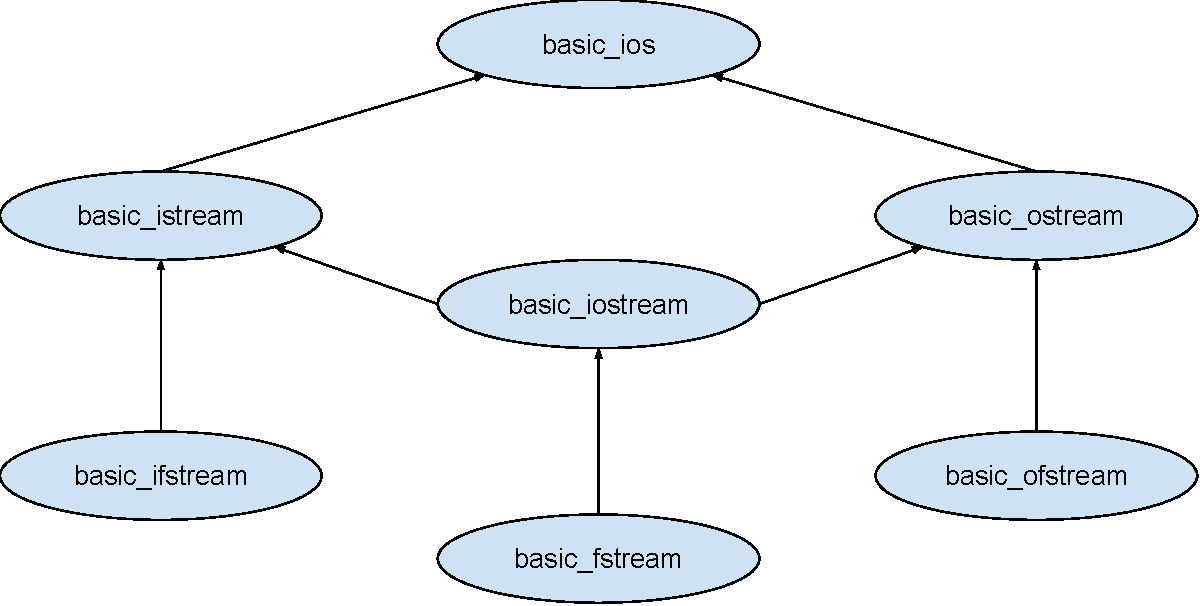
\includegraphics[width=\textwidth]{images/stream_hierarchy.pdf}
\end{frame}

\begin{frame}[fragile]
  \frametitle{Изход на поток}

  Неформатиран изход:\\[1em]
  \lst!ostream& put(char);!\\
  \lst!ostream& write(const char*, streamsize);!\\[3em]
  \pause
  Форматиран изход:\\[1em]
  \lst!ostream& operator<<(ostream&, T);! % поправка на оцветяването >>
\end{frame}

\begin{frame}[fragile]
  \frametitle{Вход от поток}

  Неформатиран вход:\\[1em]
  \lst!istream& get(char&);!\\
  \lst!istream& get(char*,streamsize,char);!\\
  \lst!istream& getline(char*,streamsize,char);!\\
  \lst!streamsize gcount() const;!\\
  \lst!istream& read(char*, streamsize);!\\[2em]
  \pause
  Форматиран вход:\\[1em]
  \lst!istream& operator>>(istream&, T&);!\\[2em]
  \pause
  Допълнителни функции:\\
  \lst!int peek();!\\
  \lst!istream& putback(char);!
\end{frame}

\begin{frame}[fragile]
  \frametitle{Низови потоци}

  \lst@#include <sstream>@\\[1em]
  Входен поток от низ: \lst{istringstream}\\[1em]
  \textbf{Пример:}
\begin{lstlisting}
char s[] = "1 2 3";
istringstream iss(s);
int a, b, c;
iss >> a >> b >> c;
\end{lstlisting}
  \vspace{1em}
  \pause
  Изходен поток към низ: \lst{ostringstream}\\[1em]
  \textbf{Пример:}
\begin{lstlisting}
ostringstream oss;
oss << 1.2 << ' ' << 3.4;
cout << oss.str();
\end{lstlisting}
\end{frame}

\begin{frame}[fragile]
  \frametitle{Състояние на поток}

  Флагове за състояние:\\[1em]
  \begin{tabular}{|c||c|c|c|c|}
    \hline
    \multirow{2}{*}{\tt{iostate}}&\tt{goodbit}&\tt{eofbit}&\tt{failbit}&\tt{badbit}\\
    \cline{2-5}
    &0&1&2&4\\
    \hline
  \end{tabular}\\[1em]
  \pause
  Селектори:\\
  \lst!bool good() const;!
  \lst!bool eof() const;!\\
  \lst!bool fail() const;!
  \lst!bool bad() const;!\\
  \lst!iostate rdstate() const;!\\[1em]
  Мутатор:\\
  \lst!void clear(iostate = 0);!\\[1em]
  \textbf{Примери:}\\
  \lst!if (cin.rdstate() & (eofbit | badbit)) ...!\\
  \lst!cin.clear(failbit);!\\
  \lst!if(cin)...!\hspace{10ex}\lst@if(!cin)...@
\end{frame}

\begin{frame}[fragile]
  \frametitle{Потокови манипулатори}

  \lst@#include<iomanip>@\\
  \lst!stream << data1 << manipulator << data2;!
  \begin{itemize}
  \item Манипулатори за изход: \lst{endl}, \lst{ends}, \lst{flush}
  \item Манипулатори за бройна система: \lst{hex}, \lst{oct}, \lst{dec}
  \item Манипулатори за поле: \lst{setw}, \lst{setfill}, \lst{left}, \lst{right}, \lst{internal}
  \item Манипулатори за дробни числа: \lst{fixed}, \lst{scientific}, \lst{setprecision}
  \item Манипулатори за формат: \lst{setiosflags}, \lst{setbase}
  \item \ldots и много други
  \end{itemize}
\end{frame}

\section{Файлове}

\begin{frame}
  \frametitle{Какво е файл?}

  \begin{itemize}[<+->]
  \item Блок информация, записана на траен носител
  \item Разлика между масив и файл
  \item Файлови системи
  \item Метаданни на файла
  \end{itemize}
\end{frame}

\begin{frame}
  \frametitle{Файлове и потоци}

  \textbf{Файлът като поток:}
  \begin{itemize}[<+->]
  \item Последователен достъп
  \item Еднопосочно обхождане
  \item Еднократна обработка
  \item Краен поток
  \item Файлът може да играе ролята на
    \begin{itemize}
    \item производител (входни файлове)
    \item консуматор (изходни файлове)
    \end{itemize}
  \end{itemize}

  \onslide<+->
  \textbf{Файлът не е само поток:}
  \begin{itemize}[<+->]
  \item Пряк достъп
  \item Разширяване при запис
  \item Едновременно четене и запис
  \end{itemize}
\end{frame}

\begin{frame}
  \frametitle{Текстови и двоични файлове}

  \textbf{Текстови файлове}
  \begin{itemize}[<+->]
  \item Форматиран вход и изход
  \item Само последователен достъп
  \item Еднократно обхождане
  \item Интерпретиране на данните във файла като текст (ASCII, Unicode или др.)
  \item Прилича на низ
  \end{itemize}

  \onslide<+->
  \textbf{Двоични файлове}
  \begin{itemize}[<+->]
  \item Неформатиран (суров) вход и изход
  \item Позволява пряк достъп
  \item Многократно обхождане
  \item Интерпретацията на данните във файла зависи от конкретната задача
    \begin{itemize}
    \item  масив от числа
    \item структура
    \item масив от структури
    \end{itemize}
  \end{itemize}
\end{frame}

\section{Файлове в C++}

\begin{frame}[fragile]
  \frametitle{Входни файлове}

  \lst!ifstream(char const*, openmode = ios::in )!\\[1em]
  \begin{itemize}
  \item \lst!void open(char const*, openmode = ios::in)!
  \item \lst!void close()!
  \item \lst!ios::binary! — суров (неформатиран) вход
  \end{itemize}
  \vspace{3em}
  \pause
  \textbf{Примери:}
\begin{lstlisting}
ifstream fi("email.txt", ios::in );
ifstream fi("lolcat.jpg", ios::in | ios::binary );
\end{lstlisting}
\end{frame}

\begin{frame}[fragile]
  \frametitle{Изходни файлове}

  \lst!ofstream(char const*, openmode = ios::out|ios::trunc)!\\[1em]
  \begin{itemize}
  \item \lst!void open(char const*, openmode)!
  \item \lst!void close()!
  \item \lst!ios::trunc! --- отрязва (унищожава) файла
  \item \lst!ios::ate! --- вмъкването става в края
  \item \lst!ios::app! --- вмъкването винаги е в края
  \end{itemize}
  \vspace{1em}
  \pause
  \textbf{Примери:}
\begin{lstlisting}
ofstream fo("page.html", ios::out );
ofstream fo("application.log", ios::out | ios::app );
ofstream fo("file.dat", ios::out | ios::binary );
\end{lstlisting}
\end{frame}

\begin{frame}[fragile]
  \frametitle{Входно-изходни файлове}

  \lst!fstream(char const*, openmode = ios::in | ios::out)!\\[3em]
  \pause
  \textbf{Пример:}
\begin{lstlisting}
fstream f( "essay.txt" );
f.getline(line, 100);
f << "Ignore the following text, please!";
\end{lstlisting}
\end{frame}

\begin{frame}[<1-2>]
  \frametitle{Файлов указател}

  \begin{tikzpicture}
    \matrix[array] {
      \tt{}%
      \&\&\&|(H)| H\& e\& l\& l\& o\& ,\&|(space)|  \& w\& o\& r\& l\& d\& !\& \textbackslash n\&\&\\
    };
    \begin{scope}[visible on=<1>]
      \pointerto{H.south}{}{below}
    \end{scope}

    \begin{scope}[visible on=<2>]
      \pointerto{space.south}{}{below}
    \end{scope}
  \end{tikzpicture}
  \pause
\end{frame}

\begin{frame}[fragile]
  \frametitle{Пряк достъп до файлове}

  Отправна точка за преместване на текущата позиция:\\
  \begin{tabular}{|c||c|c|c|}
    \hline
    seekdir&beg&cur&end\\
    \hline
  \end{tabular}\\[2em]
  Селектори:
\begin{lstlisting}
streampos tellg() const
streampos tellp() const
\end{lstlisting}
  Мутатори:
\begin{lstlisting}
istream& seekg(streampos, seekdir = beg)
ostream& seekp(streampos, seekdir = beg)
\end{lstlisting}
\end{frame}

\section{Блокови файлове}

\begin{frame}[fragile]
  \frametitle{Блокова организация}

  \begin{center}
    \newcommand{\yc}{|[fill=yellow]|}
    \makecommand{\gc}{|[fill=green]|}
    \newcommand{\byc}{\yc\&\yc\&\yc\&\yc}
    \newcommand{\bgc}{\gc\&\gc\&\gc\&\gc}
    \begin{tikzpicture}
      \pgfkeys{/pgf/number format/int detect}
      \matrix[array,nodes={minimum size=2.7ex}] (a) {
        \byc\&\bgc\&\byc\&\bgc\&\byc\&\bgc\\
      };
      \foreach \i in {1,5,...,23} {
        \tikzmath{
          int \x, \y;
          \x = 3 + \i;
          \y = 1 + \i;
        }
        \draw [thick,decoration={brace,mirror,raise=1pt},decorate] (a-1-\i.south west) -- (a-1-\x.south east);
        \node [below=1ex of a-1-\y.south east] {\small\tt{Student}};
      };
    \end{tikzpicture}
  \end{center}
\begin{lstlisting}
class Student { ... };

Student s;
f.seekp( i * sizeof (Student) );
f.write((char const*)&s, sizeof(Student));

Student sa[3];
f.seekg( j * sizeof(Student) );
f.read( (char*)sa, 3 * sizeof(Student));
\end{lstlisting}
\end{frame}

\begin{frame}
  \frametitle{Задача ``СУСИ''}

  \begin{itemize}
  \item Да се въведе списък от студенти
  \item Да се запише в текстов файл \tt{students.txt}
  \item От \tt{students.txt} да се прочетат студентите, които не са скъсани и да се запишат в главната книга \tt{main.bk}
  \item В главната книга да се повиши с 1.0 оценката на студент с даден Ф№
  \end{itemize}
\end{frame}


\end{document}
